\documentclass[preprint,12pt]{elsarticle}

\usepackage{amsmath,amssymb}
\usepackage{graphicx}
\usepackage{booktabs}
\usepackage{bm}
\usepackage[colorlinks=true,allcolors=blue]{hyperref}

\newcommand{\Rev}{\mathcal{R}}
\newcommand{\logR}{\log \Rev}
\newcommand{\rk}{r_{\kappa}}
\newcommand{\Om}{\Omega}
\newcommand{\Nof}{n_t}

\journal{Physica A}

\begin{document}

\begin{frontmatter}

\title{The Ramsey community number as a renormalization-group crossing}

\author{Alexei Vazquez}
\affiliation{organization={Nodes \& Links Ltd}, city={Cambridge}, country={United Kingdom}}

\begin{abstract}
A network must be large enough before communities emerge. The smallest size at
which a split into communities is the better description is the Ramsey community
number $\rk$. For a family of networks grown by a fixed
rule, $\rk$ has been obtained numerically. Here we report an exact calculation for the diamond hierarchical
lattice, based on real-space renormalization. One generation of growth replaces every edge by $b$ parallel paths of
$s$ edges, and acts on the edge and degree counts the comparison depends on
as an exact
linear map with two eigenvalues: a volume eigenvalue $bs$ multiplying the bulk,
and a smaller seam eigenvalue $b$ multiplying the boundary between communities,
which therefore thins at every step. Carried by that flow, the evidence per edge
tends to $\ln K$ for $K$ communities, so $\rk$ is the first generation whose
accumulated evidence clears the threshold $\ln[q/(1-q)]$ set by the required
certainty $q$. This yields a closed form $\rk(b,s;q)$ for the whole family, with
the condition under which it is exact. Conditioned on the same partition, the
plain and degree-corrected comparisons agree here up to logarithmic corrections:
the gap between them is a node-labelling prior worth $-n\ln K$ for a network of
$n$ nodes, not degree correction. On the same lattice the Reichardt--Bornholdt
community Hamiltonian has an exact community-ordered phase below the
ferromagnetic critical temperature, for every value of its resolution parameter
$\gamma>0$; its modularity-optimal refinement cuts the hierarchy at half its
depth, into $K_{\rm opt}\sim(\gamma^2n)^{1/4}$ communities, and stays thermally
rigid up to an ordering temperature $k_BT_c\to3J/(2\ln K)$, with $J$ the bond
coupling. The emergent partition is detectable, optimal, and thermodynamically
ordered.
\end{abstract}

\begin{keyword}
community detection \sep renormalization group \sep hierarchical lattices \sep
Ramsey community number \sep Potts model
\end{keyword}

\end{frontmatter}

\section{Introduction}
\label{sec:intro}

How large must a network grow before its community structure becomes an
objective fact? Communities---groups of nodes more densely wired among
themselves than to the rest of the network---are the most studied form of
mesoscopic organization in networks~\cite{fortunato2010,fortunato2016}. The
difficulty is that any sufficiently flexible algorithm will carve communities
out of a structureless graph, so the existence of a partition
returned by an algorithm is no evidence that the network has one.

The standard remedy is Bayesian model comparison~\cite{holland1983,karrer2011,
peixoto2017}. Two models are fitted to the same network. The first is a
stochastic block model: the nodes are divided into blocks, and the probability
of an edge depends only on which blocks its endpoints belong to, so the model
can express the statement ``these groups exist''. The second is a null model
with a single block, in which every node is statistically equivalent to every
other, so it cannot express that statement at all. Each model assigns a
probability to the observed network once its parameters are integrated out;
these two numbers are the \emph{evidences}, and their ratio
\begin{equation}
  \Rev = \frac{P(\text{network} \mid \text{block model})}
              {P(\text{network} \mid \text{null model})}
  \label{eq:R}
\end{equation}
says how much better the network is described with groups than without them.
Throughout, we call the block-model hypothesis ``the split''. With no prior
preference for either model, the posterior probability of the split is
\begin{equation}
  P(\text{split}) = \frac{\Rev}{1+\Rev},
  \label{eq:Psplit}
\end{equation}
and we declare the split \emph{detected} once $P(\text{split})\ge q$ at a
prescribed certainty $q$, for instance $q=0.99$. Equivalently, $\logR$ must
reach the decision threshold $\ln[q/(1-q)]$. In sparse random graphs this
competition produces a genuine phase transition in
detectability~\cite{decelle2011}.

For a deterministic family of networks that grows by a fixed local rule, the
same decision rule defines a size. Detection fails on the small members of the
family and succeeds on the large ones, and the \emph{Ramsey community
number}~\cite{d7kf-s1cf} is the smallest size at which it succeeds,
\begin{equation}
  \rk(q) \;=\; \min\{\, n : P(\text{split})\ge q \,\},
  \label{eq:rk}
\end{equation}
in the spirit of Ramsey theory, where a structure is forced to appear once a
system is large enough. A plain ring never breaks ($\rk=\infty$), while a ring
with second-neighbor bonds breaks at
$\rk\approx35$~\cite{vazquez2026ringwantsbroken}; and on the scale-free
pseudofractal web of Dorogovtsev, Goltsev and Mendes~\cite{dgm2002} the values
$1095$ and $42$ are reported for the plain and the degree-corrected
comparison~\cite{karrer2011,vazquez2026communitystructurepseudofractalweb}. In every case reported so far,
however, $\rk$ and the asymptotic growth rate $\logR\sim\sigma n$ of the
evidence were obtained numerically: the evidences are closed-form, but the
crossing and the slope are read off a curve.

In this work we show that on hierarchical lattices $\rk$ need not be read off a
curve at all: it is an exact renormalization-group (RG) statement. We work on
the diamond hierarchical lattice of Migdal and
Kadanoff~\cite{migdal1976,kadanoff1976}, the standard setting in which real-space
decimation is exact and spin models are solved by iterating a
recursion~\cite{berker1979,kaufman1981,griffiths1982}. Three results follow.
First, the quantities the two models depend on---the numbers of edges within
and between blocks and the block degree sums, which are the sufficient
statistics of the block model---are transformed by one generation of growth
through an exact \emph{linear} map, whose two eigenvalues are a volume
eigenvalue $bs$ that multiplies the bulk and a seam eigenvalue $b$ that
multiplies the community boundary, with $b$ the number of parallel branches and
$s$ the number of edges per branch in the elementary cell. Second, the evidence
ratio, which is a fixed nonlinear function of those statistics, is carried by
this flow to a \emph{community fixed point} at which the evidence per edge
equals $\ln K$, with $K$ the number of communities---a value independent of the
lattice, and the fixed-point free-energy density of the detection problem.
Third, $\rk$ is the generation at which the accumulated evidence first exceeds
the decision threshold, which we evaluate exactly and also give in closed form
for the whole $(b,s)$ family, together with the condition under which the
closed form is exact.

These detection results have a thermodynamic counterpart on the same lattice.
Because the linear map is a real-space RG recursion, we can ask whether the
community partition is not only detectable but thermodynamically ordered.
Placing the Reichardt--Bornholdt community Hamiltonian~\cite{reichardt2004},
whose ground state is the partition itself, on the diamond and solving it by
the same decimation, we find an exact community-ordered phase that survives as
$n\to\infty$. Allowing each nested sub-community its own label, the
modularity-optimal description is a hierarchy cut at half the depth of the
lattice, so the optimal number of communities grows with the lattice; and that
hierarchy remains thermally rigid below a critical temperature that falls
logarithmically with the number of communities.

Two clarifications frame what follows. First, this is a study of an exactly
solvable model, not a detection algorithm. The partition tested is prescribed
by the construction of the lattice, and no search over partitions is performed
or needed; the purpose is to expose, in a setting where every quantity is
exact, what the detectability of communities means physically. Second, the
symbol $q$ denotes the detection certainty of Eq.~\eqref{eq:rk} and nothing
else; the number of communities, and equivalently the number of states of the
Potts models of Secs.~\ref{sec:hier} and~\ref{sec:pottsT}, is always $K$.

The paper is organized as follows. Section~\ref{sec:model} defines the lattice
and the self-similar bipartition whose detectability we study, and gives its
block statistics in closed form. Section~\ref{sec:rgmap} derives the exact
linear RG map obeyed by those statistics and identifies its volume and seam
eigenvalues. Section~\ref{sec:evidence} constructs the Bayesian evidence,
states precisely which prior convention each model uses, and shows that on this
lattice the plain and degree-corrected comparisons differ only by a
node-labelling prior. Section~\ref{sec:fixedpoint} shows that the evidence
density flows to $\ln K$ and quantifies the approach to that value.
Section~\ref{sec:rk} defines $\rk$ as the exact threshold crossing, gives the
asymptotic estimate of the crossing generation, and delimits when the estimate
is exact. Section~\ref{sec:general} proves the underlying lemma, map, and
density for the whole $(b,s)$ family and derives the closed form $\rk(b,s;q)$.
Section~\ref{sec:critical} states the dictionary with critical phenomena.
Section~\ref{sec:rb} places the Reichardt--Bornholdt Hamiltonian on the lattice
and solves it exactly, identifying the ordered partition.
Section~\ref{sec:hier} finds the modularity-optimal nested hierarchy, and
Section~\ref{sec:pottsT} its finite-temperature rigidity.
Section~\ref{sec:conclusions} concludes. Appendix~\ref{app:methods} collects
the computational methods in enough detail to reproduce every number.

\section{The diamond lattice and the bundle partition}
\label{sec:model}

The aim of this section is to define the lattice, to define the bipartition
whose detectability the rest of the paper analyses, and to give in closed form
the handful of counts on which both models depend.

The $(b,s)$ diamond lattice is grown by edge replacement. Starting from a
single bond between two poles $A$ and $B$, each generation replaces every edge
by $b$ parallel paths of $s$ edges; the $s\!-\!1$ interior vertices of every
path are new (Fig.~\ref{fig:construction}). We present the standard diamond
$b=s=2$, which is also the $(2,2)$-flower of the recursive scale-free
nets~\cite{rozenfeld2007}, and give the general result where it is established.
After $t$ generations the lattice has
\begin{equation}
  m = (bs)^t = 4^t \ \text{edges}, \qquad
  \Nof = \tfrac{1}{3}\left(2\cdot 4^t + 4\right)\ \text{nodes}.
  \label{eq:sizes}
\end{equation}
A vertex born at generation $k$ has degree $2\cdot2^{\,t-k}$, and the poles are
permanent hubs of degree $b^t=2^t$: the lattice is strongly degree
heterogeneous, which is what makes the plain versus degree-corrected comparison
of Sec.~\ref{sec:evidence} nontrivial.

\begin{figure*}[tb]
  \centering
  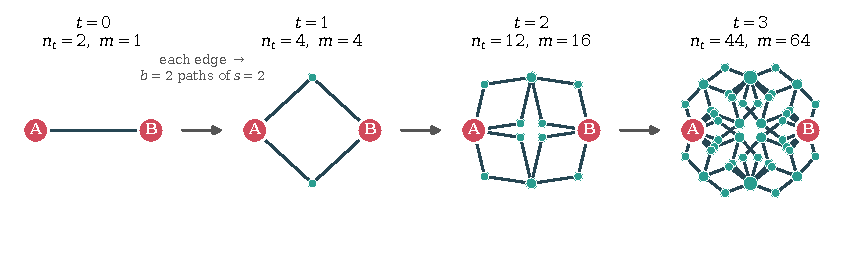
\includegraphics[width=\textwidth]{fig_construction.pdf}
  \caption{Construction of the diamond hierarchical lattice for $b=s=2$ by
  edge replacement. Starting from a single bond between the poles $A,B$
  ($t=0$), each generation replaces every edge by $b=2$ parallel paths of
  $s=2$ edges, adding one interior vertex per path; iterating gives $m=4^t$
  edges and $\Nof=(2\cdot4^t+4)/3$ nodes [Eq.~\eqref{eq:sizes}]. Node area
  $\propto$ degree, so the two poles emerge as the permanent degree-$2^t$
  hubs.}
  \label{fig:construction}
\end{figure*}

\begin{figure*}[tb]
  \centering
  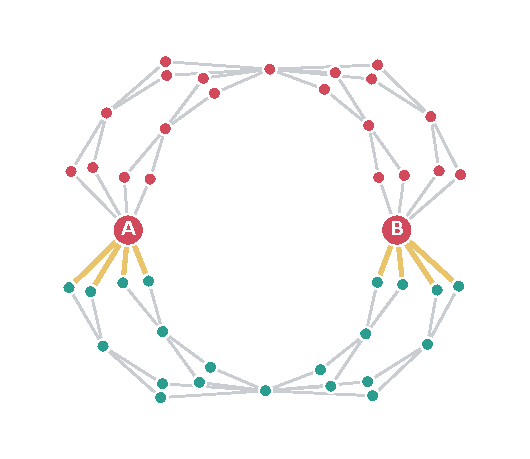
\includegraphics[width=\textwidth]{fig_lattice.pdf}
  \caption{The two top-level cuts of the diamond lattice $G_3$ ($\Nof=44$),
  which sever the same $2^t=8$ seam edges (gold), every one of them incident on
  a pole. (a)~The \emph{bundle cut} tested by the Bayesian evidence of
  Sec.~\ref{sec:evidence}: block~1 (red) is bundle~0 together with both poles
  $A,B$, block~2 (teal) is bundle~1. (b)~The \emph{staggered cut}, which
  assigns one pole to each block and is the ground state of the
  Reichardt--Bornholdt Hamiltonian of Sec.~\ref{sec:rb}. Node area $\propto$
  degree, exposing the two degree-$2^t$ hubs.}
  \label{fig:lattice}
\end{figure*}

The self-similar community structure is the pair of parallel bundles between
the poles. Label the two bundles created at $t=1$ and let every later vertex
and edge inherit the label of the edge it replaces. The bipartition we test is
block~$1=$ bundle~$0\cup\{A,B\}$, block~$2=$ bundle~$1$
[Fig.~\ref{fig:lattice}(a)], the analogue of the recursive branch cut of the
pseudofractal web~\cite{vazquez2026communitystructurepseudofractalweb}. Because
the bundles meet only at the poles, every edge of bundle~0 lies inside block~1,
and every edge crossing the cut is an edge of bundle~1 incident on a pole. Elementary counting then
gives closed forms for the block-pair statistics---$e_{rs}$ edges between
blocks $r$ and $s$, and block degree sums $\kappa_r$ with
$\kappa_1+\kappa_2=2m$:
\begin{align}
  e_{11} &= \tfrac{4^t}{2}, &
  e_{22} &= \tfrac{4^t}{2}-2^t, &
  e_{12} &= 2^t, \notag\\
  \kappa_1 &= 4^t+2^t, &
  \kappa_2 &= 4^t-2^t, &&
  \label{eq:counts}
\end{align}
verified against direct construction through $t=7$ (Table~\ref{tab:counts}).
The seam is subextensive, $e_{12}=2^t=\sqrt{m}$, so the fraction of edges
crossing the cut decays geometrically, $e_{12}/m=(1/s)^t\to0$: the two halves
become ever more cleanly separated as the lattice grows. The cut is also
nearly balanced in node number, $n_1/n_2=1+6/(4^t-1)\to1$, and in degree,
$\kappa_1/\kappa_2=1+2(1/s)^t+O(s^{-2t})\to1$; this matters in
Sec.~\ref{sec:evidence}.

\begin{table}[tb]
  \centering
  \caption{Closed-form block-pair statistics of the bundle cut,
  Eq.~\eqref{eq:counts}, verified against direct construction through $t=7$.}
  \label{tab:counts}
  \begin{tabular}{lcccccc}
    \toprule
    $t$ & $\Nof$ & $e_{11}$ & $e_{22}$ & $e_{12}$ & $\kappa_1$ & $\kappa_2$\\
    \midrule
    1 & 4    & 2    & 0    & 2  & 6    & 2   \\
    2 & 12   & 8    & 4    & 4  & 20   & 12  \\
    3 & 44   & 32   & 24   & 8  & 72   & 56  \\
    4 & 172  & 128  & 112  & 16 & 272  & 240 \\
    5 & 684  & 512  & 480  & 32 & 1056 & 992 \\
    \bottomrule
  \end{tabular}
\end{table}

\section{The renormalization-group map}
\label{sec:rgmap}

This section establishes the structural fact on which everything else rests:
growth acts on the block statistics of Eq.~\eqref{eq:counts} as an exact linear
map, and the two eigenvalues of that map separate bulk growth from the growth
of the community boundary.

Collect the statistics in the vector
$\bm v=(e_{11},e_{22},e_{12},\kappa_1,\kappa_2)^{\top}$. One generation of
growth acts \emph{exactly linearly}, $\bm v(t{+}1)=M\bm v(t)$, with
\begin{equation}
  M=\begin{pmatrix}
     4&0&0&0&0\\ 0&4&2&0&0\\ 0&0&2&0&0\\ 0&0&-2&4&0\\ 0&0&2&0&4
    \end{pmatrix}.
  \label{eq:M}
\end{equation}
Its entries have a direct physical reading. An edge inside either block is
replaced by four edges whose new interior vertices inherit its bundle label, so
within-block edges quadruple. A seam edge joins a pole (block~1) to a
bundle-1 vertex (block~2), and its new vertices carry the bundle-1 label into
block~2: of its four children, the two at the pole remain seam edges and the
two at the old block-2 endpoint are absorbed into block~2. Hence
$e_{12}'=2e_{12}$, with the displaced pair reappearing as $+2e_{12}$ in
$e_{22}'$; the degree rows follow from $\kappa_r=2e_{rr}+e_{12}$. Read
backwards, $M^{-1}$ is the Migdal--Kadanoff decimation that strips the youngest
generation; read forwards, $M$ is the growth generator of the detection
problem.

Because $M$ is triangular, its eigenvalues can be read off the diagonal. There
are two distinct ones,
\begin{equation}
  \lambda_{\rm vol}=bs=4 \quad\text{(fourfold)},
  \qquad
  \lambda_{\rm seam}=b=2 ,
  \label{eq:eigs}
\end{equation}
and they are eigenvalues of $M$ in the ordinary sense: any component of $\bm v$
along the corresponding eigenvector is multiplied by that factor at every
generation. The fourfold \emph{volume} eigenvalue $\lambda_{\rm vol}$
reproduces the growth of the edge count and of the degree sums, $m=(bs)^t$; the
single \emph{seam} eigenvalue $\lambda_{\rm seam}$ governs the community
boundary, $e_{12}=b^t$. In the symmetric cell $b=s$ the two roles cannot be
told apart from the numbers alone; the general derivation of
Sec.~\ref{sec:general} shows that the seam obeys $c_{t+1}=b\,c_t$ exactly for
all $(b,s)$, confirmed by direct construction across the family. The spectral
gap is thus
\begin{equation}
  \frac{\lambda_{\rm seam}}{\lambda_{\rm vol}} = \frac{1}{s} ,
  \label{eq:gap}
\end{equation}
set by the series length alone. For $s\ge2$ the seam is an irrelevant direction
relative to the bulk and the crossing fraction flows to zero: the cut is a
community boundary that sharpens as the lattice grows. The degenerate case $s=1$
(parallel bonds, no interior vertices) has unit gap and never separates---the
diamond analogue of the plain cycle that never
breaks~\cite{vazquez2026ringwantsbroken}. Community detectability on these
lattices is, in this precise sense, a relevant direction of the RG flow,
switched on exactly when $s\ge2$; the two control parameters play distinct
roles, $b$ setting the number of communities and $s$ the sharpness of their
separation.

\section{Bayesian evidence for the split}
\label{sec:evidence}

The aim of this section is to write down the two evidences whose ratio enters
Eq.~\eqref{eq:R} as explicit functions of the statistics of
Eq.~\eqref{eq:counts}, and---because the comparison is only meaningful if both
models are treated alike---to state exactly which prior convention each one
uses.

\subsection{The degree-corrected evidence}

The detection rule is that of the companion
works~\cite{vazquez2026ringwantsbroken,
vazquez2026communitystructurepseudofractalweb}; we recall its degree-corrected
construction in enough detail that Eq.~\eqref{eq:dc} can be read off directly.
Following Ref.~\cite{vazquez2026communitystructurepseudofractalweb}, the graph
is modeled as a Poisson multigraph with degree-corrected rates
$\langle A_{ij}\rangle=\theta_i\theta_j\,\omega_{g_ig_j}$, where
$\theta_i=k_i/\sqrt{2m}$ carries the degree of node $i$ ($2m=\sum_i k_i$) and
$g_i$ is its block. The null $\omega_{rs}\equiv1$ is then the configuration
model---random wiring at fixed degrees~\cite{karrer2011}---so that any split it
favors reflects structure beyond the degree sequence. The affinities have
configuration-model edge expectations $\Om_{rr}=\kappa_r^2/4m$ and
$\Om_{rs}=\kappa_r\kappa_s/2m$ ($r\neq s$), with $\sum_{r\le s}\Om_{rs}=m$. The
Poisson likelihood factorizes over block pairs,
$P(A\mid\omega,g)=C(A,\bm k)\prod_{r\le s}
\omega_{rs}^{\,e_{rs}}e^{-\omega_{rs}\Om_{rs}}$, and its prefactor $C(A,\bm k)$
depends only on the fixed degrees and adjacency, not on the partition; it is
this factor---the degree-only and combinatorial part---that cancels in any
evidence ratio. Placing a symmetric conjugate prior
$\omega_{rs}\sim\Gamma(\alpha,\alpha)$ (mean one, centered on the configuration
model) and integrating each affinity out leaves the marginal evidence of one
block pair,
\begin{equation}
  Z(e,\Om)=\frac{\alpha^\alpha}{\Gamma(\alpha)}\int_0^\infty\!
    \omega^{\,e+\alpha-1}e^{-(\Om+\alpha)\omega}\,d\omega
    =\frac{\alpha^\alpha}{\Gamma(\alpha)}\,
     \frac{\Gamma(e{+}\alpha)}{(\Om{+}\alpha)^{e+\alpha}} .
  \label{eq:Zdc}
\end{equation}
The evidence for the split is the product of these factors over the occupied
block pairs, divided by the single-block null---one pair comprising the whole
graph, with $e\!\to\!m$ and $\Om\!\to\!m$. Taking logarithms,
$\logR_{\rm dc}=\sum_{r\le s}\ln Z(e_{rs},\Om_{rs})-\ln Z(m,m)$, and inserting
Eq.~\eqref{eq:Zdc},
\begin{align}
  \logR_{\rm dc}
  &= \sum_{r\le s}\Big[\ln\Gamma(e_{rs}{+}\alpha)
      -(e_{rs}{+}\alpha)\ln(\Om_{rs}{+}\alpha)
      +\alpha\ln\alpha-\ln\Gamma(\alpha)\Big] \notag\\
  &\quad -\Big[\ln\Gamma(m{+}\alpha)-(m{+}\alpha)\ln(m{+}\alpha)
      +\alpha\ln\alpha-\ln\Gamma(\alpha)\Big],
  \label{eq:dc}
\end{align}
where the second bracket is the null term $\ln Z(m,m)$---the whole graph as a
single block, so that $e\!\to\!m$ and $\Om\!\to\!m$, with no cross term. The
$\alpha\ln\alpha-\ln\Gamma(\alpha)$ pieces do not fully cancel: the split sum
carries three of them (one per block pair) against the null's one, leaving a net
Occam factor $[\alpha^\alpha/\Gamma(\alpha)]^{2}$ for the two extra affinities.
For contrast we also evaluate the plain Bernoulli block model with symmetric
$B(\alpha,\alpha)$ priors on the block densities. Inserting the closed
forms~\eqref{eq:counts} makes both evidences explicit functions of $t$; all
evaluations use 80-digit arithmetic and match direct construction of the
lattice exactly (Appendix~\ref{app:methods}).

\subsection{Prior conventions, and what degree correction does here}
\label{sec:priors}

Both evidences above are \emph{conditional on the prescribed bundle partition}:
the block assignment $g$ is fixed by the construction of the lattice, no prior
over partitions is included, and no search over partitions is performed. This
is the convention in which the fixed-point density of
Sec.~\ref{sec:fixedpoint} is defined, and we use it throughout as the primary
convention. It is the appropriate one here because the partition is not an
inference target: the question asked is whether \emph{this} partition describes
the network better than none.

A second convention appears in the companion
works~\cite{vazquez2026ringwantsbroken,
vazquez2026communitystructurepseudofractalweb}, where the plain-model evidence
carries in addition a node-labelling prior, obtained by integrating a
Beta--Bernoulli membership probability over the two blocks. It contributes the
factor
\begin{equation}
  \Lambda_t = \ln B(n_1{+}\alpha,n_2{+}\alpha)-\ln B(\alpha,n{+}\alpha)
            = -\,n\ln K + O(\ln n),
  \label{eq:label}
\end{equation}
the log prior odds of the prescribed labelling against the all-in-one-block
labelling; for a balanced $K$-way split of $n$ nodes it is the cost $-n\ln K$
of naming which block each node belongs to. Numerically $\Lambda_t/(-n\ln2)
=0.999999$ at $t=12$ (Table~\ref{tab:conventions}). Because $\Lambda_t$ is
extensive in $n$ while the evidence is extensive in $m$, and $n/m\to2/3$ on
this lattice, the labelling prior does not merely shift the evidence: it
rescales its density.

Putting both models in both conventions makes the comparison unambiguous
(Table~\ref{tab:conventions}). Two facts emerge. (i) Within a convention, the
plain and degree-corrected evidences agree to $O(\ln m)$: their difference is
$-1.5$, $-11.5$ and $-22.5$ at $t=4,8,12$, against evidences of order
$10^2$, $10^4$ and $10^7$. The reason is visible in Eq.~\eqref{eq:counts}: the
bundle cut is balanced both in node number, $n_1/n_2\to1$, and in degree,
$\kappa_1/\kappa_2\to1$, so the configuration-model expectations $\Om_{rs}$ and
the plain model's $n_rn_s$ expectations are proportional, and degree correction
has nothing to remove. Consequently degree correction does not move $\rk$ at
all on this lattice (Table~\ref{tab:rk}). This need not hold in general: on a
lattice whose blocks differ in their degree distributions the two models are
genuinely different, and a much larger separation between them is reported for
the pseudofractal web~\cite{vazquez2026communitystructurepseudofractalweb};
the present calculation shows only that the two effects must be separated
before either is credited with the difference, and that on the diamond the
difference is entirely the labelling prior. (ii) On this
lattice the whole gap between the ``plain'' and the ``degree-corrected'' curve
is $\Lambda_t$. In the labelled convention both densities converge to
\begin{equation}
  \frac{\logR}{m}\ \longrightarrow\ \Big(1-\frac{n}{m}\Big)\ln K ,
  \label{eq:labelled_density}
\end{equation}
i.e.\ $\ln 2/3=0.2310$ here (measured slope $0.2302$ between $t=12$ and
$t=13$), against $\ln2$ in the conditional convention. The ratio of the two
densities is therefore $(1-n/m)^{-1}$: exactly $3$ for the diamond, where
$n/m\to2/3$, and $2$ for a lattice with $n/m\to1/2$ such as the pseudofractal
web---which is precisely the factor of two reported
there~\cite{vazquez2026communitystructurepseudofractalweb}. That factor is thus fixed
by the node-to-edge ratio and the labelling prior, not by degree correction. All statements below use
the conditional convention unless stated otherwise, and none of the RG results
depend on the choice: $\Lambda_t$ is a fixed function of $n$ that shifts the
threshold crossing without touching the map $M$, its eigenvalues, or the flow.

\begin{table}[tb]
  \centering
  \caption{The two prior conventions at $\alpha=1$. Conditional on the
  prescribed partition, the plain and degree-corrected evidences agree to
  $O(\ln m)$ and both have density $\ln K=\ln 2$. Adding the node-labelling
  prior $\Lambda_t\to-n\ln K$ of Eq.~\eqref{eq:label} to either model reduces
  the density to $(1-n/m)\ln K=\ln2/3$ and delays the crossing by two
  generations. The last two columns are the same two models with that prior
  included, and they too agree to $O(\ln m)$.}
  \label{tab:conventions}
  \footnotesize
  \setlength{\tabcolsep}{4pt}
  \begin{tabular}{lrrrrrr}
    \toprule
    & & \multicolumn{2}{c}{conditional} & &
    \multicolumn{2}{c}{with labelling prior}\\
    \cmidrule(lr){3-4}\cmidrule(lr){6-7}
    $t$ & $\Nof$ & $\logR_{\rm dc}$ & $\logR_{\rm pl}$ & $\Lambda_t$
        & $\logR_{\rm dc}{+}\Lambda_t$ & $\logR_{\rm pl}{+}\Lambda_t$\\
    \midrule
    2  & 12       & $0.03$   & $1.08$   & $-6.67$    & $-6.64$   & $-5.60$\\
    3  & 44       & $16.32$  & $16.56$  & $-28.33$   & $-12.01$  & $-11.77$\\
    4  & 172      & $111.9$  & $110.4$  & $-116.4$   & $-4.55$   & $-6.04$\\
    5  & 684      & $559.9$  & $556.2$  & $-470.6$   & $89.26$   & $85.55$\\
    6  & 2732     & $2500$   & $2494$   & $-1890$    & $610.7$   & $604.5$\\
    8  & 43692    & $43738$  & $43727$  & $-30279$   & $13459$   & $13447$\\
    10 & 699052   & $718680$ & $718663$ & $-484539$  & $234141$  & $234124$\\
    12 & $1.12{\times}10^{7}$ & $1.1591{\times}10^{7}$ & $1.1591{\times}10^{7}$
       & $-7.753{\times}10^{6}$ & $3.838{\times}10^{6}$
       & $3.838{\times}10^{6}$\\
    \midrule
    \multicolumn{2}{l}{density $\logR/m\to$}
       & $\ln2$ & $\ln2$ & & $\ln2/3$ & $\ln2/3$\\
    \bottomrule
  \end{tabular}
\end{table}

\begin{figure*}[tb]
  \centering
  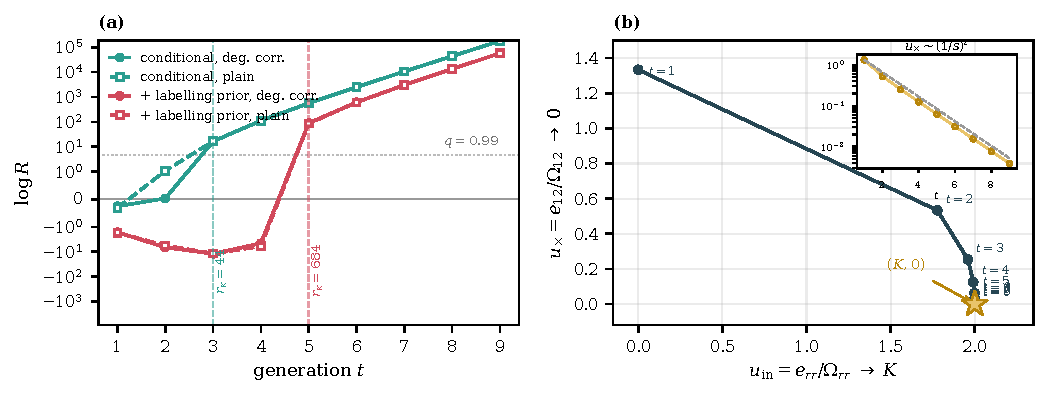
\includegraphics[width=1\textwidth]{fig_data.pdf}
  \caption{(a) Log evidence of the bundle split versus generation (symlog
  scale) for both models in both prior conventions. Within a convention the
  plain and degree-corrected curves are indistinguishable on this scale; the
  two conventions are separated by the node-labelling prior $\Lambda_t$ of
  Eq.~\eqref{eq:label}. The conditional evidences clear the detection threshold
  $\ln[q/(1{-}q)]$ (dotted, $q=0.99$) at $t=3$, giving $\rk=n_3=44$; with the
  labelling prior included the crossing moves to $t=5$, $\rk=n_5=684$. The
  lattice exists only at the discrete sizes $\Nof$, so the crossing---and hence
  $\rk$---is a generation index. (b) Renormalization-group flow of the block
  densities Eq.~\eqref{eq:densities} to the community fixed point
  $(u_{\rm in},u_{\times})=(K,0)=(2,0)$; the seam density decays geometrically
  as $(\lambda_{\rm seam}/\lambda_{\rm vol})^t=(1/s)^t$ (inset).}
  \label{fig:data}
\end{figure*}

\section{The fixed-point evidence density}
\label{sec:fixedpoint}

This section shows where the flow of Sec.~\ref{sec:rgmap} takes the evidence:
to a fixed point at which the evidence per edge is a pure number, $\ln K$, and
quantifies how fast that value is approached.

Because $\bm v$ flows under $M$ with dominant rate $bs$ and $\logR_{\rm dc}$ is
a fixed function of $\bm v$, the evidence is carried by the flow, and its
leading behavior is transparent. For large counts,
$\ln\Gamma(e{+}\alpha)-(e{+}\alpha)\ln(\Om{+}\alpha)=e\ln(e/\Om)-e+O(\ln e)$,
and the $-e$ terms cancel against the null since $\sum_{r\le s}e_{rs}=m$. What
survives is the degree-corrected surprise
$\logR_{\rm dc}=\sum_{r\le s}e_{rs}\ln(e_{rs}/\Om_{rs})+O(\ln m)$---the
Kullback--Leibler divergence between the observed and the
configuration-expected edge placement, the quantity a degree-corrected modularity
estimates~\cite{newman2006}. Its natural variables are the running block
densities
\begin{equation}
  u_{\rm in}=\frac{e_{rr}}{\Om_{rr}}=\frac{2x^2}{(x\pm1)^2},
  \qquad
  u_{\times}=\frac{e_{12}}{\Om_{12}}=\frac{2x}{x^2-1},
  \label{eq:densities}
\end{equation}
with $x=2^t$. Under the flow they converge to the \emph{community fixed point}
\begin{equation}
  (u_{\rm in},\,u_{\times}) \;\longrightarrow\; (K,\,0) = (2,\,0),
  \label{eq:fp}
\end{equation}
the seam density decaying as
$(\lambda_{\rm seam}/\lambda_{\rm vol})^t=(1/s)^t$
[Fig.~\ref{fig:data}(b)]. At the fixed point each within-block term contributes
$\tfrac{m}{2}\ln K$ and the cross term is subleading, so the evidence density
converges to a pure number,
\begin{equation}
  \boxed{\ \frac{\logR_{\rm dc}}{m}\ \longrightarrow\ \ln K\ }
  \label{eq:lnK}
\end{equation}
The interpretation is information-theoretic. For $K$ equal, well-separated
communities, $e_{rr}=m/K$ while the configuration model expects
$\Om_{rr}=m/K^2$; hence $u_{\rm in}=K$ identically, and each edge contributes
exactly $\ln K$---the entropy of resolving which of $K$ communities it belongs
to. The value is therefore independent of the lattice, and indeed the symmetric
three-community cut of the pseudofractal web obeys $e_{rr}/\Om_{rr}\to3$ with
density $\ln3$~\cite{vazquez2026communitystructurepseudofractalweb}.

By the \emph{detection problem} we mean, throughout, the comparison of the two models
of Eqs.~\eqref{eq:R}--\eqref{eq:Psplit} on this family of lattices, regarded as
a statistical-mechanics problem in its own right: $\logR$ plays the role of a
free energy, the statistics $\bm v$ the role of couplings, and $M$ the role of
the RG recursion. In that dictionary Eq.~\eqref{eq:lnK} is its fixed-point
free-energy density.

Table~\ref{tab:density} makes the convergence explicit and tests it against the
analytic correction derived in Sec.~\ref{sec:general}. Writing
$\logR_{\rm dc}/m=(\ln K)(1-\delta_t)$, the deficit measured from the exact
evidence and the prediction
$\delta_t\simeq\frac{2(b-1)}{b\ln b}\frac{t\ln s+1}{s^{t}}$ of
Eq.~\eqref{eq:delta} agree to four significant figures by $t=12$ and better
beyond, and the density reaches $0.693133$ against $\ln2=0.693147$ at $t=20$.
The approach to $\ln K$ is thus accounted for by the seam mode of the RG map:
the deficit is the price of the $b^t$
crossing edges still present at generation $t$, and it decays at the rate set
by the spectral gap $1/s$.

\begin{table}[tb]
  \centering
  \caption{Convergence of the evidence density to $\ln K=\ln2=0.693147$
  ($\alpha=1$, conditional convention). $\delta_t^{\rm exact}=
  1-\logR_{\rm dc}/(m\ln2)$ is the measured deficit and $\delta_t$ the
  prediction of Eq.~\eqref{eq:delta}; their ratio tends to $1$.}
  \label{tab:density}
  \begin{tabular}{rrrrrr}
    \toprule
    $t$ & $m$ & $\logR_{\rm dc}/m$ & $\delta_t^{\rm exact}$ & $\delta_t$
        & ratio\\
    \midrule
    3  & $64$                  & $0.255053$ & $0.632036$ & $0.555337$ & $1.1381$\\
    4  & $256$                 & $0.436965$ & $0.369593$ & $0.340168$ & $1.0865$\\
    5  & $1024$                & $0.546755$ & $0.211199$ & $0.201334$ & $1.0490$\\
    6  & $4096$                & $0.610401$ & $0.119378$ & $0.116292$ & $1.0265$\\
    8  & $6.55{\times}10^{4}$  & $0.667393$ & $0.037155$ & $0.036886$ & $1.0073$\\
    10 & $1.05{\times}10^{6}$  & $0.685387$ & $0.011196$ & $0.011175$ & $1.0019$\\
    12 & $1.68{\times}10^{7}$  & $0.690871$ & $0.003284$ & $0.003282$ & $1.0005$\\
    14 & $2.68{\times}10^{8}$  & $0.692494$ & $0.000943$ & $0.000943$ & $1.0001$\\
    16 & $4.29{\times}10^{9}$  & $0.692963$ & $0.000266$ & $0.000266$ & $1.0000$\\
    20 & $1.10{\times}10^{12}$ & $0.693133$ & $0.000020$ & $0.000020$ & $1.0000$\\
    \bottomrule
  \end{tabular}
\end{table}

The early generations behave differently. At $t=1$ block~2 is a single
edgeless vertex, $u_{\rm in}^{(2)}=0$, and the trajectory in
Fig.~\ref{fig:data}(b) starts far from the fixed point; there the surprise is
small and the $O(\ln m)$ remainder of Eq.~\eqref{eq:dc}---the Occam cost of
the extra block affinities---dominates, making $\logR_{\rm dc}$ negative: the
partition is the more complex hypothesis, and it is rejected until the
structural term outweighs that cost. Since the seam mode decays by $1/s$ per
generation, the densities converge to $(K,0)$ within a few generations and the extensive $\ln K$ term takes over. Prior
insensitivity follows likewise: $\alpha$ enters only through the $O(\ln m)$
Occam terms.

\section{The Ramsey community number}
\label{sec:rk}

The aim of this section is to define $\rk$ on this lattice as an exact
threshold crossing, to give the asymptotic estimate of the crossing generation
that follows from Eq.~\eqref{eq:lnK}, and to be explicit about the difference
between the two.

\subsection{The exact crossing}

The rule $P(\text{split})\ge q$ reads $\logR\ge\ln[q/(1{-}q)]$, and since the
lattice exists only at the discrete sizes $\Nof$, $\rk$ is the first generation
to clear the threshold:
\begin{equation}
  \rk(q)=\Nof\big|_{t_\star}, \qquad
  t_\star=\min\Big\{t:\logR_{\rm dc}(t)\ge L\Big\},
  \qquad L=\ln\frac{q}{1-q}.
  \label{eq:cross}
\end{equation}
Equation~\eqref{eq:cross} is the definition, and it is exact: $\logR_{\rm dc}$
is known in closed form at every $t$ from Eqs.~\eqref{eq:counts}
and~\eqref{eq:dc}, so $t_\star$ is obtained by evaluating a known function on
the integers, with no fitting and no asymptotics. This is the precise sense in
which $\rk$ is an RG crossing: it is the generation at which the running,
extensive evidence---driven by the volume eigenvalue once the flow has turned
onto the community fixed point---first exceeds a fixed detection threshold.
Evaluated this way [Fig.~\ref{fig:data}(a), Table~\ref{tab:rk}], the
conditional evidence gives $\rk=12$ at $q=0.5$ and $\rk=44$ from $q=0.9$ all
the way to $q=0.999$: a sharp, $\alpha$-independent step, because the evidence
jumps between discrete sizes. Including the labelling prior moves both models
to $\rk=684$ over the same range. Degree correction, by contrast, does not move
$\rk$ at all here, for the reason given in Sec.~\ref{sec:priors}.

\begin{table}[tb]
  \centering
  \caption{Ramsey community number $\rk(q)=\Nof|_{t_\star}$ for the bundle cut
  ($\alpha=1$), from the exact crossing Eq.~\eqref{eq:cross}. Within a prior
  convention the plain and degree-corrected models give the same answer; the
  two conventions differ by two generations.}
  \label{tab:rk}
  \begin{tabular}{lcccc}
    \toprule
    & \multicolumn{2}{c}{conditional} &
      \multicolumn{2}{c}{with labelling prior}\\
    \cmidrule(lr){2-3}\cmidrule(lr){4-5}
    $q$ & degree corrected & plain & degree corrected & plain\\
    \midrule
    $0.5$          & $n_2=12$ & $n_2=12$ & $n_5=684$ & $n_5=684$\\
    $0.9$--$0.999$ & $n_3=44$ & $n_3=44$ & $n_5=684$ & $n_5=684$\\
    \bottomrule
  \end{tabular}
\end{table}

\subsection{The asymptotic estimate and when it is exact}
\label{sec:asymptotic}

Equation~\eqref{eq:lnK} suggests a closed-form shortcut. Replacing
$\logR_{\rm dc}(t)$ by its asymptotic form $(\ln K)(bs)^t$ and solving for the
first integer that clears $L$ gives
\begin{equation}
  t_\star \simeq \Big\lceil
    \log_{bs}\frac{L}{\ln K}
  \Big\rceil .
  \label{eq:tstar}
\end{equation}
Equation~\eqref{eq:tstar} is an \emph{estimate}, not an identity: it uses the
fixed-point density in place of the exact evidence and therefore ignores the
deficit $\delta_t$ of Eq.~\eqref{eq:delta} and the $O(\ln m)$ Occam terms. It
holds when the crossing occurs in the asymptotic regime, and fails otherwise,
in three identifiable ways.

\emph{(i) Near threshold.} By Eq.~\eqref{eq:delta} the exact crossing generation
equals Eq.~\eqref{eq:tstar} whenever
$L\le(1-\delta_{t_\star})(\ln K)(bs)^{t_\star}$, and is larger otherwise. The
window in which the estimate fails has relative width $\delta_{t_\star}\sim
t_\star\ln s/s^{t_\star}$ and closes as $L$ grows. Table~\ref{tab:validity}
gives the comparison across the family: for $L\gtrsim10^5$
Eq.~\eqref{eq:tstar} is exact for every lattice tested, whereas at the
practically interesting certainties $q=0.99$ and $q=0.999$ ($L=4.6$ and $6.9$)
it misses for most of them, by one generation and, when the crossing happens in
the first few generations, by two. The largest $L$ at which we find a miss is
$5.6\times10^2$ for $(2,2)$, $1.3\times10^2$ for $(2,3)$, and
$4.2\times10^4$ for $(4,2)$.

\emph{(ii) At $q=1/2$.} The threshold is $L=0$ and the argument of the
logarithm in Eq.~\eqref{eq:tstar} vanishes, so the estimate is undefined
($t_\star\to-\infty$). This is not a removable singularity but a statement
about the physics: at $q=1/2$ the crossing is decided not by the extensive
$\ln K$ term at all but by the sign change of the $O(\ln m)$ Occam remainder
during the transient, that is, by the generation at which the structural term
first outweighs the complexity cost. The exact rule Eq.~\eqref{eq:cross} handles this without
modification and gives $t_\star=2$ for every member of the family we have
examined ($\logR_{\rm dc}=-0.25$ at $t=1$ and $+0.03$ at $t=2$ for the
diamond), hence $\rk=n_2$: for $(b,s)=(2,2),(3,2),(4,2),(2,3),(2,4),(3,3)$ this
is $\rk=12,23,38,30,56,62$. For any $q<1/2$ the threshold is negative and
$t_\star$ is smaller still. Equation~\eqref{eq:tstar} should therefore be used
only for $q>1/2$, and quantitatively only for $L\gg\ln K$.

\emph{(iii) Finite-size corrections in general.} Even above threshold the exact
evidence carries the deficit $\delta_t$; the closed form
Eq.~\eqref{eq:rkbs} below should be read as the leading behavior of an
expression whose correction is known and given in Eq.~\eqref{eq:delta}.

\begin{table}[tb]
  \centering
  \caption{Asymptotic estimate against exact crossing across the $(b,s)$
  family: entries are $t_\star$ from Eq.~\eqref{eq:tstar} / $t_\star$ from the
  exact rule Eq.~\eqref{eq:cross}, at threshold $L=\ln[q/(1-q)]$. Boldface
  marks disagreement. The estimate is exact for every lattice once
  $L\gtrsim10^5$, and unreliable at the certainties used in practice.}
  \label{tab:validity}
  \begin{tabular}{lcccccc}
    \toprule
    & \multicolumn{2}{c}{practical $q$} & \multicolumn{4}{c}{large $L$}\\
    \cmidrule(lr){2-3}\cmidrule(lr){4-7}
    $(b,s)$ & $L=4.6$ & $L=6.9$ & $10^2$ & $10^3$ & $10^5$ & $10^7$\\
    \midrule
    $(2,2)$ & \textbf{2/3} & \textbf{2/3} & 4/4 & 6/6 & 9/9 & 12/12\\
    $(3,2)$ & \textbf{1/3} & \textbf{2/3} & 3/3 & \textbf{4/5} & 7/7 & 9/9\\
    $(4,2)$ & \textbf{1/2} & \textbf{1/2} & 3/3 & 4/4 & 6/6 & 8/8\\
    $(2,3)$ & 2/2 & 2/2 & 3/3 & 5/5 & 7/7 & 10/10\\
    $(2,4)$ & \textbf{1/2} & 2/2 & 3/3 & 4/4 & 6/6 & 8/8\\
    $(3,3)$ & \textbf{1/2} & \textbf{1/2} & 3/3 & 4/4 & 6/6 & 8/8\\
    \bottomrule
  \end{tabular}
\end{table}

\subsection{Two readings of $\rk$}
\label{sec:tworeadings}

Two readings of $\rk$ have so far been used interchangeably. The first is \emph{the crossing}: the smallest
member of the family whose exact evidence clears the threshold,
Eq.~\eqref{eq:cross}. The second is \emph{the slope}: extract the asymptotic
growth rate $\sigma$ of $\logR$ by fitting the large-$n$ behavior, then invert
$\sigma n=L$ to place the crossing. The results above show that these are not
equivalent, and in what way.

The slope reading is asymptotically correct---indeed we can now dispense with
the fit altogether, since Eq.~\eqref{eq:lnK} \emph{derives} the slope,
$\sigma=\ln K$ per edge, with no free parameters---but as a way of locating
$\rk$ it is quantitatively wrong in the regime used in practice.
Table~\ref{tab:validity} shows the discrepancy: at $q=0.99$ the slope-based
estimate places the crossing of the diamond at $t_\star=2$ ($n=12$) where the
exact rule gives $t_\star=3$ ($n=44$), a factor of nearly four in size; for
$(3,2)$ the error is two generations, a factor $(bs)^2=36$ in the number of
edges and $131/5\approx26$ in the number of nodes. The reason is
Table~\ref{tab:density}: at the generations where a practical threshold is
crossed the evidence density is still far below $\ln K$---short by $63\%$ at
$t=3$ and $37\%$ at $t=4$---so an asymptotic slope systematically overestimates
the accumulated evidence and therefore underestimates $\rk$. The two readings converge only for
$L\gtrsim10^5$, that is, for certainties $1-q\lesssim e^{-10^5}$, which no
application requires. We therefore take Eq.~\eqref{eq:cross}, evaluated on the
exact evidence, as the definition of $\rk$, and Eqs.~\eqref{eq:tstar}
and~\eqref{eq:rkbs} as its asymptotic form with a known correction.

\section{The general \texorpdfstring{$(b,s)$}{(b,s)} family}
\label{sec:general}

The aim of this section is to prove for the whole $(b,s)$ family what
Secs.~\ref{sec:model}--\ref{sec:rk} established for the standard diamond: the
bundle structure, the linear map and its spectrum, the fixed-point density
$\ln K=\ln b$, and the closed form of the crossing generation with its
finite-size correction.

With $n_t=2+b(s{-}1)[(bs)^t{-}1]/(bs{-}1)$ nodes at generation $t$,
Eq.~\eqref{eq:tstar} at $K=b$ gives the asymptotic closed form
\begin{align}
  \rk(b,s;q) &= 2+\frac{b(s{-}1)}{bs-1}\Big[(bs)^{t_\star}-1\Big],
  \label{eq:rkbs}\\
  t_\star &= \Big\lceil \log_{bs}\!\Big(\ln\tfrac{q}{1-q}\Big/\ln b\Big)
  \Big\rceil ,\notag
\end{align}
subject to the validity conditions of Sec.~\ref{sec:asymptotic}. Here $b$
enters through the entropy accumulated per edge and $s$ through the volume
growth, while degrees, priors, and lattice details drop out. We now derive this
form, and the exact linear map and fixed-point density on which it rests.

\subsection{Bundle lemma}
Label the $b$ paths created at $t=1$ as bundles
$0,\dots,b{-}1$, and let every vertex and edge created later inherit the
bundle label of the edge it replaces. We claim that, at every generation and
for $s\ge2$, each edge either has both endpoints interior to a single bundle
or joins a pole to a bundle vertex; no edge ever joins two distinct bundles.
This holds at $t=1$, where the bundles are internally disjoint paths sharing
only the poles. Inductively, replacing an edge creates $s\!-\!1$ interior
vertices per path, all carrying the parent's bundle label, and every child
edge joins two vertices from the set \{parent endpoints, new vertices\}; since
the parent's endpoints belong to one bundle (or are poles) and the new
vertices inherit its label, no child can bridge two bundles. $\square$

\subsection{Per-bundle statistics and the linear map}
By the lemma, all
block-pair statistics of the $K{=}b$ bundle partition (block $0=$ bundle $0\cup
\{A,B\}$, block $r=$ bundle $r$) are linear in two per-bundle counts: the
pole-incident edges $c_t$ and the interior edges $i_t$ of one bundle. Under
one generation, a pole-incident edge spawns $b$ paths, each contributing
exactly one new pole-incident edge and $s\!-\!1$ interior edges, while an
interior edge spawns $bs$ interior edges:
\begin{equation}
  c_{t+1}=b\,c_t, \qquad i_{t+1}=bs\,i_t+b(s{-}1)\,c_t .
  \label{eq:recbs}
\end{equation}
The map is triangular, so its spectrum is read off the diagonal:
$\lambda_{\rm vol}=bs$ and $\lambda_{\rm seam}=b$, proving
the spectrum of Eq.~\eqref{eq:eigs} for all $(b,s)$. With the initial condition
of a single path per bundle, $c_1=2$, $i_1=s-2$, the solution is
\begin{equation}
  c_t=2\,b^{\,t-1}, \qquad i_t=b^{\,t-1}\!\left(s^t-2\right)
  \qquad (s\ge2).
  \label{eq:icbs}
\end{equation}
The block statistics follow by the lemma: $e_{00}=i_t+c_t=b^{\,t-1}s^t$,
$e_{rr}=i_t$ and $e_{0r}=c_t$ for $r\ge1$, and $e_{rs}=0$ for $r\neq s\ge1$;
the block degree sums are $\kappa_r=2i_t+c_t=2b^{\,t-1}(s^t{-}1)$ and
$\kappa_0=\kappa_r+b\,c_t=2b^{\,t-1}(s^t{-}1{+}b)$; and since each replaced
edge adds $b(s{-}1)$ vertices, $n_t=2+b(s{-}1)[(bs)^t{-}1]/(bs{-}1)$. All of
these, including $e_{rs}=0$, were checked against direct construction for
$(b,s)$ with $b\le4$, $s\le5$. The $b=s=2$ specialization reproduces
Eqs.~\eqref{eq:counts} and~\eqref{eq:M} (there block $2$ collects the second
bundle, $e_{22}=i_t$, $e_{12}=c_t$).

\subsection{Densities and the fixed point}
Writing $x=s^t$, the configuration
ratios are exact rational functions,
\begin{align}
  \frac{e_{00}}{\Om_{00}} &= \frac{b\,x^2}{(x{+}b{-}1)^2}, &
  \frac{e_{rr}}{\Om_{rr}} &= \frac{b\,x(x{-}2)}{(x{-}1)^2}, \notag\\
  \frac{e_{0r}}{\Om_{0r}} &= \frac{b\,x}{(x{-}1)(x{+}b{-}1)}
  &&\xrightarrow{\ t\to\infty\ } \frac{b}{s^t},
  \label{eq:ratiosbs}
\end{align}
so both within-block densities flow to $u_{\rm in}=b=K$ and the seam density
to zero as $(1/s)^t$, establishing the community fixed point $(K,0)$ for the
whole family.

\subsection{Evidence density and its correction}
Insert Eq.~\eqref{eq:ratiosbs} into the surprise form of the evidence,
\begin{equation}
  \logR_{\rm dc}=\sum_{r\le s}e_{rs}\ln\frac{e_{rs}}{\Om_{rs}}+O(\ln m);
  \label{eq:surprise}
\end{equation}
the empty
pairs $e_{rs}=0$ ($r\neq s\ge1$) contribute only their Occam terms,
$O(b^2\ln m)$. Because every ratio in Eq.~\eqref{eq:ratiosbs} carries the same
prefactor $b$ and $\sum_{r\le s}e_{rs}=m$, the $\ln b$ contributions sum to
$m\ln b$ \emph{exactly}; expanding the residual logarithms in $1/x$ gives
\begin{align}
  \logR_{\rm dc} &= m\ln b\left[\,1-\delta_t\,\right],
  \label{eq:delta}\\
  \delta_t &= \frac{2(b{-}1)}{b\ln b}\,\frac{t\ln s+1}{s^{t}}
  +O\!\Big(\frac{t}{s^{2t}}\Big),\notag
\end{align}
up to the $O(m^{-1}\ln m)$ Occam terms. The dominant deficit is the seam's:
$e_{0r}\ln(e_{0r}/\Om_{0r})\simeq -c_t\,t\ln s$ per pair, i.e., the price of
the $b^t$ crossing edges still present at generation $t$. Numerically the
ratio of the exact deficit to Eq.~\eqref{eq:delta} is $1.027$, $1.002$,
$1.0001$ at $t=6,10,14$ for $(b,s)=(2,2)$ (Table~\ref{tab:density}), and
analogously across the family.

\subsection{Validity of the crossing formula}
By Eq.~\eqref{eq:delta} the exact crossing generation equals the ceiling formula
of Eq.~\eqref{eq:rkbs} whenever $L\le(1-\delta_{t_\star})\,(\ln b)(bs)^{t_\star}$,
and exceeds it otherwise; in the asymptotic regime the excess is exactly one
generation, while for crossings that occur in the first two or three
generations it can be two, as tabulated in Table~\ref{tab:validity}. The
misfire window has relative width $\delta_{t_\star}\sim t_\star\ln
s/s^{t_\star}$ and vanishes as $q\to1$. Both regimes occur: for
$(b,s)=(2,2)$ the formula is exact at every decade $10^3\le L\le10^8$, while
for $(3,2)$ at $L=10^3$ the evidence at the predicted generation is $994.1$,
just short, and the crossing lands one generation later---precisely the
mechanism quantified by Eq.~\eqref{eq:delta}.

\section{Connection to critical phenomena}
\label{sec:critical}

This short section states the dictionary that the rest of the paper exploits.
The correspondence with critical phenomena on these
lattices~\cite{migdal1976,kadanoff1976,berker1979,kaufman1981,griffiths1982} is
direct: the sufficient statistics are the couplings, $M$ is the recursion, the
volume and seam eigenvalues are the bulk and interfacial rescaling factors,
detectability is a relevant direction of the flow for $s\ge2$, and $\ln K$ is
the fixed-point free-energy density. The correspondence is not merely formal:
on the same lattice one can place a spin model whose ground state is the
community partition itself, and ask whether community order survives
thermally---which we take up next.

\section{A thermodynamic community-ordered phase}
\label{sec:rb}

The aim of this section is to show that the community partition is the ground
state of a genuine spin model on this lattice, to identify which partition that
is, and to show by exact solution that it supports a thermodynamic ordered
phase that persists as $n\to\infty$.

The natural Hamiltonian is that of Reichardt and
Bornholdt~\cite{reichardt2004}, whose minimization is community detection and
which reduces to modularity at unit resolution,
\begin{equation}
  \mathcal{H} = -\sum_{i\neq j}\big(A_{ij}-\gamma\,p_{ij}\big)\,
                \delta(\sigma_i,\sigma_j),
  \label{eq:rbH}
\end{equation}
with $A_{ij}$ the adjacency matrix, $\sigma_i\in\{1,\dots,K\}$ the community
label, $\gamma$ a resolution parameter, and $p_{ij}=\kappa_i\kappa_j/2m$ the
configuration null. We take the Ising case $K=2$, $\sigma_i=\pm1$. Using
$\delta(\sigma_i,\sigma_j)=\tfrac12(1+\sigma_i\sigma_j)$ and dropping constants,
Eq.~\eqref{eq:rbH} becomes a ferromagnet on the graph edges plus an
infinite-range, degree-weighted antiferromagnetic penalty,
\begin{equation}
  \mathcal{H} = -\!\sum_{\langle ij\rangle}\!\sigma_i\sigma_j
    \;+\;\frac{\gamma}{4m}\,\Big[M_\kappa^2-\!\sum_i\kappa_i^2\Big],
    \qquad M_\kappa=\sum_i \kappa_i\sigma_i .
  \label{eq:rbIsing}
\end{equation}

\begin{figure*}[t]
  \centering
  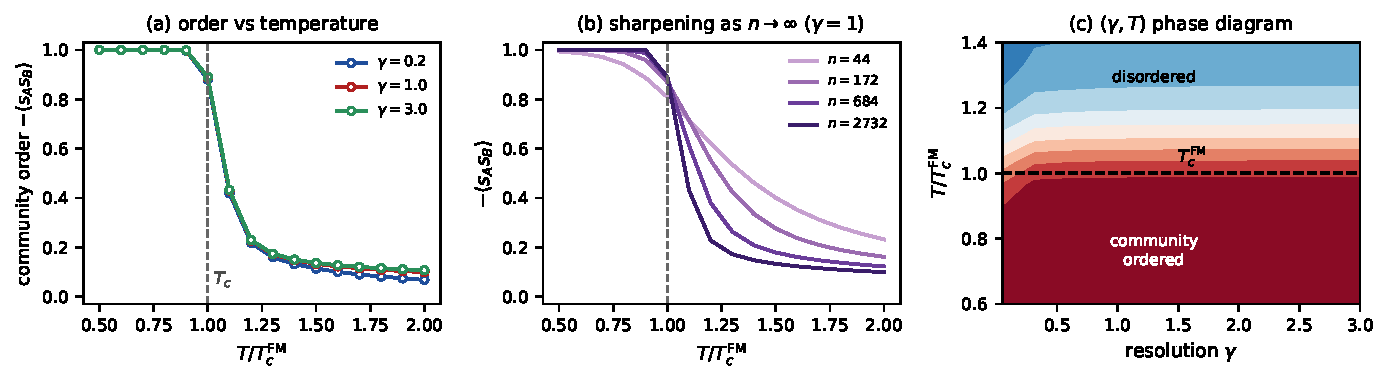
\includegraphics[width=1\textwidth]{fig_rb.pdf}
  \caption{\textbf{Exact community-ordered phase of the $K=2$
  Reichardt--Bornholdt model on the diamond.} Order parameter
  $-\langle\sigma_A\sigma_B\rangle$ (hub anti-alignment: $1$ when the two hubs
  occupy opposite communities, as in the staggered cut of
  Fig.~\ref{fig:lattice}(b)). (a)~Versus temperature at $t=6$ ($\Nof=2732$)
  for three resolutions $\gamma$: the community order switches off at the
  ferromagnetic critical temperature $T_c^{\rm FM}$, essentially independent of
  $\gamma$. (b)~As the lattice grows the transition sharpens into a step at
  $T_c^{\rm FM}$; below it the order is persistent, $-\langle\sigma_A\sigma_B
  \rangle\to1$ as $n\to\infty$. (c)~The $(\gamma,T)$ phase diagram: a
  community-ordered region for all $\gamma>0$ below $T_c^{\rm FM}$ (dashed).}
  \label{fig:rb}
\end{figure*}

The first term favors a single community (all spins aligned); the second
penalizes any net degree-weighted magnetization, and so favors a
\emph{balanced bipartition}. The resolution $\gamma$ sets the balance between
them.

\subsection{Which partition is the ground state}
\label{sec:gs}

The penalty selects a different top-level cut from the one the evidence tests,
and it is worth being explicit about which, because it is the origin of the
hub anti-alignment reported below. Two bipartitions sever exactly the same
$c_t=2^t$ seam edges (Fig.~\ref{fig:lattice}):
\begin{itemize}
\item the \emph{bundle cut} of Sec.~\ref{sec:model}, block~1$=$bundle~0
      $\cup\{A,B\}$, which puts both hubs in one block and therefore carries a
      degree imbalance $M_\kappa=\kappa_1-\kappa_2=2^{\,t+1}$;
\item the \emph{staggered cut}, block~1$=$bundle~0$\cup\{A\}$,
      block~2$=$bundle~1$\cup\{B\}$, which gives one hub to each block and is
      exactly degree balanced, $M_\kappa=0$, since each block then carries
      $\kappa=2\,i_t+c_t+b^t=m$.
\end{itemize}
The two have identical ferromagnetic energy, so from Eq.~\eqref{eq:rbIsing}
their energies differ by exactly the penalty,
\begin{equation}
  \mathcal{H}_{\rm bundle}-\mathcal{H}_{\rm stag}
  = \frac{\gamma}{4m}\big(2^{\,t+1}\big)^2 = \gamma ,
  \label{eq:gsgap}
\end{equation}
independently of size. The staggered cut is therefore the lower of the two for
every $\gamma>0$, and brute-force minimization over all $2^{n-1}$ bipartitions
at $t=2$ confirms that it is the global ground state (energy $-9.5$ at
$\gamma=1$, against $-8.5$ for the bundle cut and $-1.5$ for the single
community); Eq.~\eqref{eq:gsgap} is verified by direct construction through
$t=7$. Note that the preference is $O(1)$, not extensive: an arbitrarily small
resolution suffices to select the staggered cut, but the two cuts remain
degenerate to leading order in the size, which is why the detection analysis of
Secs.~\ref{sec:evidence}--\ref{sec:rk}---which is insensitive to an $O(1)$
relabelling of two vertices---applies to either.

\subsection{Exact solution and the ordered phase}

Because the penalty couples the spins only through the single collective
variable $M_\kappa$, the model is exactly solvable: the ferromagnetic part is
local and handled by the same decimation as above, while the value of
$M_\kappa$ is tracked by an auxiliary weight, giving the partition function as a
sum over generation-resolved edge configurations at $80$-digit precision
(Appendix~\ref{app:rbising}). We verified the solution against direct
enumeration through $t=3$.

The order parameter is the community assignment of the two hubs: the pole
correlation $\langle\sigma_A\sigma_B\rangle$, which is $+1$ when the poles share
a community (the ferromagnet, one community) and $-1$ when they are split into
opposite communities (the staggered cut of Sec.~\ref{sec:gs}). The exact
solution gives a sharp transition (Fig.~\ref{fig:rb}). Below the ferromagnetic
critical temperature $T_c^{\rm FM}$ ($k_BT_c^{\rm FM}/J=1.641$) the two hubs
lock into \emph{opposite} communities, $-\langle\sigma_A\sigma_B\rangle\to1$,
and this holds for \emph{any} resolution $\gamma>0$---even infinitesimal
$\gamma$ drives the split, exactly as Eq.~\eqref{eq:gsgap} predicts, because
flipping a hub is the single largest change available to $M_\kappa$ and the
penalty acts most strongly there. As the lattice grows the order parameter
sharpens into a step at $T_c^{\rm FM}$ [Fig.~\ref{fig:rb}(b)]: below it the
community order is \emph{persistent}, $-\langle\sigma_A\sigma_B\rangle\to1$ as
$n\to\infty$; above it the order decays to zero. The community-ordering
temperature coincides with $T_c^{\rm FM}$ and is essentially
$\gamma$-independent [Fig.~\ref{fig:rb}(c)]---the resolution selects
\emph{which} partition orders, not \emph{whether} it does. This division of
labor between the ferromagnetic part, which sets the transition temperature,
and the penalty, which selects the ordered state, is what allows the
generalization to $K>2$ in Sec.~\ref{sec:pottsT}.

This is the thermodynamic counterpart of the detection result. A purely
ferromagnetic Ising model on the diamond has no such phase---its ground state is
the trivial single community, and any community-staggered order parameter
averages to zero. The Reichardt--Bornholdt penalty changes the ground state
itself to the balanced partition, and the self-similar geometry then makes that
partition thermodynamically stable in the limit of large size: the emergent
communities are not merely detectable at $\rk$, they order.

\section{Hierarchical community structure and a growing number of states}
\label{sec:hier}

The aim of this section is to show that the two-community cut is only the top of
a self-similar tree, and to find how deep the tree should be cut---that is, how
many communities best describe the lattice.

Because the diamond is built by recursion, the same argument that favors
splitting the whole lattice favors splitting each bundle again, and the
Reichardt--Bornholdt functional keeps improving as the partition is
refined---provided each nested sub-community is given its \emph{own} label, so
that the number of Potts states grows with the depth of the hierarchy. At depth
$d$ the lattice is cut along the seams of generations $1,\dots,d$ into $K=2^{d}$
blocks, and Eq.~\eqref{eq:rbH} is evaluated with $K=2^d$ states.

The energetics are exactly solvable. Removing the depth-$d$ seams cuts
\begin{equation}
  c(d) = 2^{\,t+d}\quad(d\ge1),\qquad
  \frac{e_{\rm in}}{m}=1-2^{\,d-t},
  \label{eq:cutd}
\end{equation}
edges---each deeper level doubles the interface, exactly the seam eigenvalue
$\lambda_{\rm seam}=b=2$ acting once per level---while the degree-weighted
penalty of the $2^d$ blocks is $\sum_c\kappa_c^2/(2m)^2\to2^{-d}$ as
$t\to\infty$, dominated by the block that still holds the two hubs. The
modularity of the depth-$d$ partition is therefore, to leading order in large
size,
\begin{equation}
  Q(d) = \frac{e_{\rm in}}{m}-\gamma\,\frac{\sum_c\kappa_c^2}{(2m)^2}
       = 1 - 2^{\,d-t} - \gamma\,2^{-d} + O(2^{-t}).
  \label{eq:Qd}
\end{equation}
The two competing terms are the price of the cut, $2^{d-t}$, growing with
resolution, and the reward for balancing degree, $\gamma\,2^{-d}$, shrinking
with it. Maximizing Eq.~\eqref{eq:Qd} over $d$ gives $2^{2d}=\gamma\,2^{t}$,
i.e.\ an optimal depth
\begin{equation}
  d_\star = \tfrac12\big(t+\log_2\gamma\big),
  \label{eq:dstar}
\end{equation}
with maximal modularity $Q_\star = 1 - 2\sqrt{\gamma}\,2^{-t/2}\to1$. The
optimal cut is thus at \emph{half the depth of the lattice}, a statement that
involves neither $n$ nor $m$. The corresponding number of
communities is
\begin{equation}
  K_{\rm opt}=2^{d_\star}=\sqrt{\gamma}\;2^{t/2}
             =\sqrt{\gamma\,b^{t}}
             =\sqrt{\gamma}\;m^{1/4}
             \simeq\sqrt{\gamma}\,(3n/2)^{1/4},
  \label{eq:Kopt}
\end{equation}
where the third form is the useful one: $b^t$ is the size of the top-level
seam, and equivalently the degree of the hubs, so the optimal number of
communities is the geometric mean of the resolution and the interface. In terms
of the network size this is a quarter power, $K_{\rm opt}\sim n^{1/4}$, with
blocks of $\sim n^{3/4}$ nodes each; a least-squares fit of $\ln K_{\rm opt}$
against $\ln n$ over the five largest sizes gives a slope of $0.250$
[Fig.~\ref{fig:hier}(b)], against $1/4$ from Eq.~\eqref{eq:Kopt}. We confirm
$d_\star=\lfloor t/2\rfloor$ at $\gamma=1$ by exact construction through $t=9$.
The number of Potts states that optimally describes the network therefore grows
with the network without bound, as $n^{1/4}$.

This is the diamond counterpart of the growing-$K$ hierarchy of the
pseudofractal web~\cite{vazquez2026communitystructurepseudofractalweb}, reached
here inside a spin model: the resolution $\gamma$ sets the depth through
Eq.~\eqref{eq:dstar}, each level adds an interface that costs one factor of the
seam eigenvalue, and the single bundle cut of Sec.~\ref{sec:rb} is recovered as
the $d=1$ top of the tree. The exponent relating $K_{\rm opt}$ to $n$ is not
itself universal---it follows from Eq.~\eqref{eq:dstar} together with the
lattice's own relation between $b^t$ and $n$, which is $b^t=\sqrt{m}\sim
\sqrt{n}$ here---whereas the midpoint rule $d_\star=t/2$ at $\gamma=1$ contains
no lattice-specific quantity at all. The Ramsey community number marks where the
first level of this hierarchy becomes detectable; the deeper levels switch on,
one after another, as the lattice continues to grow.

\begin{figure}[tb]
  \centering
  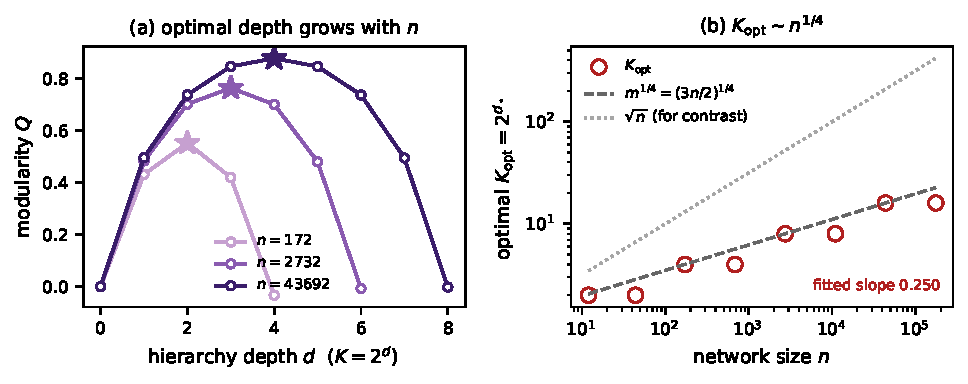
\includegraphics[width=\columnwidth]{fig_hier.pdf}
  \caption{\textbf{Hierarchical community structure with a growing number of
  states.} (a)~Modularity $Q$ of the depth-$d$ nested partition
  ($K=2^d$ communities), Eq.~\eqref{eq:Qd}, versus depth for three sizes; stars
  mark the optimum, which moves to finer resolution as $n$ grows. (b)~The
  optimal number of communities $K_{\rm opt}=2^{d_\star}$ against size, with
  the prediction $m^{1/4}=(3n/2)^{1/4}$ of Eq.~\eqref{eq:Kopt} (dashed) and,
  for contrast, $\sqrt{n}$ (dotted). The fitted slope over the five largest
  sizes is $0.250$, i.e.\ $K_{\rm opt}\sim n^{1/4}$.}
  \label{fig:hier}
\end{figure}

\section{Finite-temperature order of the hierarchy}
\label{sec:pottsT}

The aim of this section is to ask whether the nested hierarchy of
Sec.~\ref{sec:hier} survives thermally, as the two-block order of
Sec.~\ref{sec:rb} did, and to determine how its ordering temperature depends on
the number of communities.

\subsection{What is computed, and why}

Section~\ref{sec:rb} established a division of labor in Eq.~\eqref{eq:rbIsing}
that we now exploit: the degree-weighted penalty selects \emph{which} colouring
is the ground state---the balanced, staggered one---while the ferromagnetic
term, which is local, sets the temperature at which any colouring becomes
rigid. At $K=2$ both parts were treated exactly and the ordering temperature
was found to coincide with the ferromagnetic $T_c^{\rm FM}$ for all $\gamma>0$
[Fig.~\ref{fig:rb}(c)]. For the depth-$d$ hierarchy with $K=2^d$ colours we
therefore compute the rigidity of the colour field from the ferromagnetic
$K$-state Potts model on the same lattice, having established in
Sec.~\ref{sec:hier} that the RB energy at resolution $\gamma$ selects the
depth-$d_\star$ partition as its ground state. Equation~\eqref{eq:pottsRG}
below is exactly that local ferromagnetic recursion, and it does not contain
the penalty; the penalty enters the argument only through the ground-state
selection of Secs.~\ref{sec:gs} and~\ref{sec:hier}. The infinite-range term is
thus not decimated, and does not need to be, since it does not move $T_c$.

A Potts bond is described by a same-colour weight $A$ and a different-colour
weight $B$, and one generation acts by the exact series and parallel laws
\begin{equation}
\begin{aligned}
  A_{\rm ser} &= A_1A_2 + (K{-}1)B_1B_2, \\
  B_{\rm ser} &= A_1B_2 + B_1A_2 + (K{-}2)B_1B_2,
\end{aligned}
\qquad
\begin{aligned}
  A_{\rm par} &= A_1A_2,\\
  B_{\rm par} &= B_1B_2,
\end{aligned}
  \label{eq:pottsRG}
\end{equation}
so that, with $r=B/A$, one generation of the diamond is the single exact map
\begin{equation}
  r' = f(r) = \left[\frac{2r+(K{-}2)r^2}{1+(K{-}1)r^2}\right]^{2},
  \label{eq:rmap}
\end{equation}
and every finite-temperature quantity below follows from it in closed form at
every size. The order parameter is the hub--hub colour rigidity
\begin{equation}
  \rho_K = \frac{P(\sigma_A=\sigma_B)-1/K}{1-1/K},
  \label{eq:rho}
\end{equation}
the correlation of the two poles in excess of chance: $\rho_K\to1$ when the
colour field is rigid across the whole lattice and $\rho_K\to0$ when it is not.

\subsection{The transition is continuous; the step is finite size}

The results are collected in Fig.~\ref{fig:potts} and Table~\ref{tab:potts}.
The unstable fixed point $r_\star(K)$ of Eq.~\eqref{eq:rmap} gives the critical
coupling $J/k_BT_c=-\ln r_\star$, and its derivative
$\lambda_T=f'(r_\star)$ is the thermal eigenvalue, with correlation-length
exponent $\nu=\ln s/\ln\lambda_T$.

The order parameter $\rho_K(T)$ steepens into a step as the lattice grows, for
every $K$ [Fig.~\ref{fig:potts}(a)]. That steepening is a finite-size effect
and not the first-order jump familiar from the Potts model on Bravais lattices:
two exact diagnostics show that the transition is continuous for every $K$
here.
\begin{enumerate}
\item \emph{The width is finite size.} The $10$--$90\%$ width of the step,
      measured in units of the critical coupling, shrinks geometrically with
      generation at exactly the rate $\lambda_T^{-t}$
      [Fig.~\ref{fig:potts}(b)]: measured ratios per generation are $1.677$,
      $1.852$, $2.045$, $2.250$ for $K=2,4,8,16$ against
      $\lambda_T=1.679$, $1.853$, $2.045$, $2.250$. This is ordinary
      finite-size scaling at a continuous transition, with $\Delta K/K_c\sim
      L^{-1/\nu}$, and it occurs at $K=2$---known to be continuous---exactly as
      it does at $K=16$.
\item \emph{There is no latent heat.} The energy density, taken as the fraction
      of same-colour bonds $\epsilon=(1/m)\,\partial\ln Z/\partial(J/k_BT)$ and
      computed by propagating derivatives through Eq.~\eqref{eq:rmap}, is
      continuous through $T_c$ for every $K$: with $t=18$ fixed and the window
      $\pm\delta$ around $K_c$ shrinking as $10^{-2},10^{-3},10^{-4}$, the
      difference $\epsilon(K_c^+)-\epsilon(K_c^-)$ falls as
      $0.010,0.001,0.0001$ at $K=2$ and $0.118,0.026,0.005$ at $K=16$---to zero
      in every case, rather than to a finite latent heat.
\end{enumerate}
Below $T_c(K)$ the colour field is therefore rigid and the imposed partition
survives thermal noise completely as $n\to\infty$; above it the colours
decorrelate. The transition is continuous, with a $K$-dependent thermal
eigenvalue and an exponent $\nu(K)$ that decreases from $1.338$ at $K=2$ toward
$1/2$ at large $K$.

\begin{table}[tb]
  \centering
  \caption{Critical fixed point of the $K$-state Potts model on the diamond,
  from Eq.~\eqref{eq:rmap}: unstable fixed point $r_\star$, thermal eigenvalue
  $\lambda_T=f'(r_\star)$, exponent $\nu=\ln2/\ln\lambda_T$, critical coupling
  and temperature. As $K\to\infty$, $r_\star\to K^{-2/3}$ exactly, so
  $J/k_BT_c\to\tfrac23\ln K$ and $\lambda_T\to bs=4$, $\nu\to1/2$.}
  \label{tab:potts}
  \begin{tabular}{rrrrrrr}
    \toprule
    $K$ & $r_\star$ & $\lambda_T$ & $\nu$ & $J/k_BT_c$ & $k_BT_c/J$
        & $(J/k_BT_c)/\ln K$\\
    \midrule
    $2$        & $0.295598$ & $1.6786$ & $1.3383$ & $1.21876$  & $0.82051$ & $1.7583$\\
    $3$        & $0.250000$ & $1.7778$ & $1.2047$ & $1.38629$  & $0.72135$ & $1.2619$\\
    $4$        & $0.220333$ & $1.8526$ & $1.1242$ & $1.51262$  & $0.66111$ & $1.0911$\\
    $8$        & $0.158759$ & $2.0454$ & $0.9687$ & $1.84037$  & $0.54337$ & $0.8850$\\
    $16$       & $0.111111$ & $2.2500$ & $0.8548$ & $2.19722$  & $0.45512$ & $0.7925$\\
    $64$       & $0.050901$ & $2.6629$ & $0.7077$ & $2.97787$  & $0.33581$ & $0.7160$\\
    $256$      & $0.021960$ & $3.0341$ & $0.6245$ & $3.81852$  & $0.26188$ & $0.6886$\\
    $10^{5}$   & $0.000457$ & $3.8342$ & $0.5157$ & $7.69000$  & $0.13004$ & $0.6679$\\
    $10^{10}$  & $2.15{\times}10^{-7}$ & $3.9963$ & $0.5003$ & $15.35088$ & $0.06514$ & $0.6667$\\
    \bottomrule
  \end{tabular}
\end{table}

\subsection{How the ordering temperature falls with depth}

As the hierarchy deepens the transition temperature falls. Setting $r$ small in
Eq.~\eqref{eq:rmap}, the fixed-point condition becomes $K^2r^4=r$ at leading
order, so
\begin{equation}
  r_\star \to K^{-2/3},
  \qquad
  \frac{k_BT_c(K)}{J}\;\longrightarrow\;\frac{3}{2\ln K},
  \qquad
  \lambda_T\to bs=4 ,
  \label{eq:TcK}
\end{equation}
an exact asymptote rather than a fitted one; Table~\ref{tab:potts} shows
$(J/k_BT_c)/\ln K$ approaching $2/3$ from above, reaching $0.6667$ at
$K=10^{10}$, and Fig.~\ref{fig:potts}(c) shows the approach. Along the optimal
locus $K_{\rm opt}\sim m^{1/4}$ of Sec.~\ref{sec:hier} this gives
$k_BT_c/J\to 6/\ln m\sim1/\ln n$: the deepest resolvable communities order only
at the lowest temperatures, while the coarse top-level split orders first and
remains ordered over the widest range. The hierarchy thus orders level by
level, each finer level becoming rigid at a lower temperature, and every level
that is thermodynamically stable stays ordered as $n\to\infty$.

The community structure of the diamond therefore has a complete thermodynamic
counterpart. It is detectable above the Ramsey community number $\rk$
(Sec.~\ref{sec:rk}); its coarsest split is the ground state of the
Reichardt--Bornholdt Hamiltonian and orders below $T_c^{\rm FM}$
(Sec.~\ref{sec:rb}); the optimal partition is a nested hierarchy cut at half
the depth of the lattice (Sec.~\ref{sec:hier}); and that hierarchy orders
thermally, level by level, with ordering temperatures falling as $3/(2\ln K)$.
The emergent partition is not a statistical artifact but a genuine, and
persistent, form of order.

\begin{figure}[tb]
  \centering
  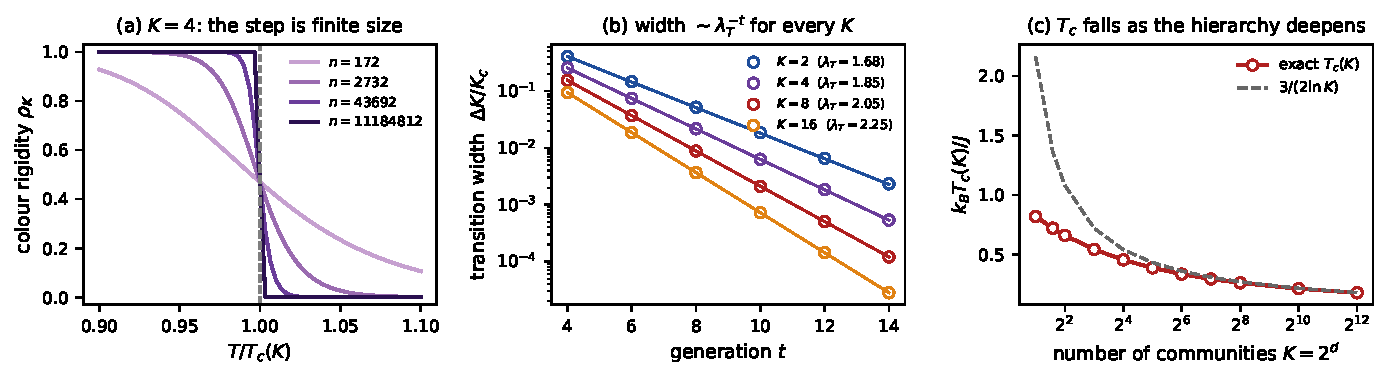
\includegraphics[width=\columnwidth]{fig_potts.pdf}
  \caption{\textbf{Finite-temperature order of the growing-$K$ hierarchy.}
  (a)~Colour rigidity $\rho_K$ of Eq.~\eqref{eq:rho} versus $T/T_c(K)$ at
  $K=4$ for four sizes: the curve steepens into a step as $n$ grows.
  (b)~The $10$--$90\%$ width of that step, in units of the critical coupling,
  against generation for $K=2,4,8,16$ (symbols) together with the finite-size
  scaling prediction $\lambda_T^{-t}$ (lines), with $\lambda_T$ the thermal
  eigenvalue of Table~\ref{tab:potts}. The step is a finite-size crossover at a
  continuous transition for every $K$, including $K=2$. (c)~The ordering
  temperature falls as the hierarchy deepens, approaching the exact asymptote
  $k_BT_c/J=3/(2\ln K)$ (dashed) of Eq.~\eqref{eq:TcK}.}
  \label{fig:potts}
\end{figure}

\section{Conclusions}
\label{sec:conclusions}

We have computed the Ramsey community number $\rk$ on the diamond hierarchical
lattice, where every quantity involved is exact. The results are as follows.

The block statistics of the bundle partition obey an exact linear map $M$ with a
volume eigenvalue $bs$ and a seam eigenvalue $b$ (Sec.~\ref{sec:rgmap}). The
evidence density is carried by this flow to $\ln K$ per edge at the community
fixed point (Sec.~\ref{sec:fixedpoint}), and $\rk$ is the first generation at
which the accumulated evidence clears the detection threshold
(Sec.~\ref{sec:rk}). It is therefore computed rather than fitted, and a closed
form holds for the whole $(b,s)$ family (Sec.~\ref{sec:general}). That closed
form is asymptotic: it reproduces the exact crossing only for
$L=\ln[q/(1-q)]\gtrsim10^5$, and at the certainties used in practice it
underestimates $\rk$ by one or two generations, because the evidence density is
then still $37$--$63\%$ short of $\ln K$ (Secs.~\ref{sec:asymptotic}
and~\ref{sec:tworeadings}). Conditioned on the same partition, the plain and
the degree-corrected evidence agree to $O(\ln m)$ and give the same $\rk$,
because the bundle cut is balanced in node number and in degree; the two curves
are separated by the node-labelling prior alone, worth $n\ln K$, and the ratio
of the evidence densities with and without that prior is $(1-n/m)^{-1}$, which
takes the value $2$ on a lattice with $n/m\to1/2$ such as the pseudofractal
web~\cite{vazquez2026communitystructurepseudofractalweb}
(Sec.~\ref{sec:priors}).

The same lattice carries a thermodynamic counterpart. The ground state of the
Reichardt--Bornholdt Hamiltonian is the staggered cut, lower than the bundle cut
by exactly $\gamma$ at every size (Sec.~\ref{sec:gs}). Below the ferromagnetic
critical temperature the two hubs occupy opposite communities, and the order
persists as $n\to\infty$, for every resolution $\gamma>0$ (Sec.~\ref{sec:rb}).
The modularity-optimal refinement is a nested hierarchy cut at half the depth of
the lattice, with $K_{\rm opt}=\sqrt{\gamma}\,m^{1/4}$ communities
(Sec.~\ref{sec:hier}), and each level orders at its own temperature, with
$k_BT_c/J\to3/(2\ln K)$. That transition is continuous for every $K$: the
sharpening of the order parameter with size is finite-size scaling of width
$\lambda_T^{-t}$, and the energy density carries no latent heat
(Sec.~\ref{sec:pottsT}).

Several directions follow. The nested hierarchy found here has its optimal cut
at half the depth of the lattice, a statement free of lattice-specific
quantities, and it would be worth proving at the level of the full partition
free energy whether that midpoint rule holds for self-similar graphs generally,
with the relation between depth and node number---and hence the exponent in
$K_{\rm opt}\sim n^{1/4}$ here---left to the individual construction.
Apollonian networks and the $(u,v)$-flowers~\cite{rozenfeld2007} carry the same
construction and would map $\rk$ across branching numbers.

The largest open question is what survives away from the deterministic lattice,
and it is really a family of questions rather than one. Disorder can enter in
several distinct ways, and they are not equivalent. Bond disorder---random
couplings on an otherwise exact hierarchical lattice---leaves the recursion
structure intact but promotes the couplings to distributions, so that $M$ acts
on distributions rather than numbers and the seam eigenvalue becomes a typical
rather than an exact rate; the Migdal--Kadanoff scheme handles this case and it
is the natural first step. Structural disorder in the growth rule---each edge
replaced by a random number of branches, or by branches of random
length---randomizes $b$ and $s$ themselves, so that $\lambda_{\rm vol}$ and
$\lambda_{\rm seam}$ become the growth rates of a multiplicative process and
one should ask whether the evidence density still self-averages to $\ln K$.
Genuinely random graphs with planted communities are further still: there the
lattice provides no exact decimation, detectability is itself a sharp phase
transition in the sparse limit~\cite{decelle2011}, and the question is whether
the crossing picture of Eq.~\eqref{eq:cross}---a running evidence with a
computable density meeting a fixed threshold---survives on average, with $\ln
K$ replaced by the corresponding annealed or quenched density. We regard the
first two as tractable extensions of the present method and the third as the
substantive open problem; establishing which features of the RG reading of
$\rk$ carry across them is what would turn this exactly solvable case into a
general theory.

\appendix

\section{Computational methods}
\label{app:methods}

Every number reported above is either a closed form or the output of an exact
recursion evaluated in multiple-precision arithmetic; none involves sampling or
fitting, except the least-squares slope quoted in Sec.~\ref{sec:hier} for
Fig.~\ref{fig:hier}(b). This appendix gives the three constructions in enough
detail to reproduce them. The accompanying scripts named below implement
exactly these steps.

\subsection{Statistics and evidence}
\label{app:evidence}

The lattice is built explicitly by edge replacement (\texttt{diamond\_rg.py},
function \texttt{diamond}) for $t\le7$ at $b=s=2$ and for $b\le4$, $s\le5$ at
$t\le4$; block-pair counts are accumulated directly from the constructed graph
and compared with Eqs.~\eqref{eq:counts} and~\eqref{eq:icbs}. Evidences are
evaluated from Eq.~\eqref{eq:dc} and its Bernoulli counterpart with
\texttt{mpmath} at $80$ decimal digits, which is required because
$\ln\Gamma(e{+}\alpha)$ and $(e{+}\alpha)\ln(\Om{+}\alpha)$ are individually of
order $m\ln m$ and cancel to order $m$. Closed-form and directly constructed
evidences agree to $10^{-6}$ at every size tested. The labelling prior of
Eq.~\eqref{eq:label} is evaluated in the same arithmetic
(\texttt{label\_prior}); switching conventions amounts to adding or omitting
that single term, which is how Table~\ref{tab:conventions} is produced.

\subsection{The $K=2$ Reichardt--Bornholdt model}
\label{app:rbising}

The penalty in Eq.~\eqref{eq:rbIsing} is infinite-range but depends on the
configuration only through the integer $M_\kappa=\sum_i\kappa_i\sigma_i$. We
therefore compute the ferromagnetic partition function \emph{resolved by} the
value of $M_\kappa$, and apply the penalty afterwards:
\begin{equation}
  Z=\sum_{M} G(M)\,
    \exp\!\Big[-\frac{\beta\gamma}{4m}\Big(M^2-\sum_i\kappa_i^2\Big)\Big],
  \qquad
  G(M)=\!\!\sum_{\{\sigma\}:\,M_\kappa=M}\!\! e^{\,\beta\sum_{\langle ij\rangle}
       \sigma_i\sigma_j}.
  \label{eq:gf}
\end{equation}
$G(M)$ is obtained by the same decimation that solves the ferromagnet, with the
bond weight promoted from a number to a polynomial in a formal variable $z$
that tracks $M_\kappa$. Concretely, the two-terminal weight of a height-$h$
sub-diamond is a $2\times2$ array $W_h(\sigma_A,\sigma_B)$ whose entries are
dictionaries $\{M\mapsto\text{weight}\}$; the recursion is
\begin{enumerate}
\item \emph{series}: join two height-$(h{-}1)$ objects through an internal spin
      of degree $2^{h}$ (the degree that spin will have in the final lattice,
      fixed at birth by its generation), summing over its two states and
      multiplying the two dictionaries by convolution in $M$, with the internal
      spin contributing $z^{\pm2^{h}}$;
\item \emph{parallel}: convolve the two resulting bundles in $M$, since their
      internal spins are independent;
\item finally attach the two poles, each of degree $2^t$, and sum over their
      four state combinations---keeping them resolved gives the pole
      correlation $\langle\sigma_A\sigma_B\rangle$ directly.
\end{enumerate}
Because the degrees are all powers of two, $M$ runs over a bounded integer grid
of step $2$, and the dictionaries stay small enough to reach $t=6$
($n=2732$). The implementation (\texttt{rb\_exact\_gf.py}, and
\texttt{rb\_fast.py} with per-generation rescaling and log-domain
accumulation) was validated against brute-force enumeration over all $2^n$
configurations at $t\le3$ and cross-validated between the two implementations
at $t=4$. Nothing is approximated: the penalty is applied exactly to each
$M$-sector. The ground-state statements of Sec.~\ref{sec:gs}, including
Eq.~\eqref{eq:gsgap}, are checked separately by exhaustive minimization at
$t=2$ and by direct evaluation of the two candidate cuts through $t=7$
(\texttt{rb\_groundstate.py}).

\subsection{The $K$-state Potts hierarchy}
\label{app:potts}

For $K>2$ we solve the ferromagnetic $K$-state Potts model exactly by the
same decimation, in the reduced variable $r=B/A$ of Eq.~\eqref{eq:rmap}
(\texttt{potts\_fixedpoint.py}). Three quantities are extracted:
\begin{itemize}
\item \emph{the critical point}, as the unstable fixed point $r_\star$ of
      Eq.~\eqref{eq:rmap} located by bisection on $f(r)-r$ at $50$ digits, with
      $\lambda_T=f'(r_\star)$;
\item \emph{the order parameter} $\rho_K$ of Eq.~\eqref{eq:rho}, from the
      unreduced pair $(A,B)$ iterated $t$ times and evaluated as
      $P(\sigma_A=\sigma_B)=A/[A+(K{-}1)B]$;
\item \emph{the energy density} $\epsilon$, by propagating $\partial/\partial
      (J/k_BT)$ analytically through the recursion alongside $(\ln A,r)$, which
      keeps the calculation stable at any depth---the values quoted in
      Sec.~\ref{sec:pottsT} use $t=18$, i.e.\ $m=6.9\times10^{10}$ edges.
\end{itemize}
As emphasized in Sec.~\ref{sec:pottsT}, this recursion contains the
ferromagnetic part of Eq.~\eqref{eq:rbH} only; the degree-weighted penalty
enters the argument through ground-state selection, not through the recursion,
and at $K=2$---where both are treated exactly by the method of
Appendix~\ref{app:rbising}---the ordering temperature is the ferromagnetic one
for every $\gamma>0$, which is what licenses this separation.

\section*{Acknowledgements}
The calculations, computer scripts, and text of this manuscript were generated
with the assistance of Claude Opus~4.8/5 (Anthropic).

\vspace{4pt}
\bibliographystyle{elsarticle-num}
\bibliography{refs}

\end{document}
